\documentclass[a4paper]{report}
\usepackage[utf8]{inputenc}
\usepackage[T1]{fontenc}
\usepackage[francais]{babel}
\usepackage{listings}
\usepackage{color}
\usepackage{listingsutf8}
\usepackage[pdftex]{graphicx}
\usepackage{float}
\usepackage{titlesec}
\usepackage{fullpage}
\usepackage{pdfpages}
\usepackage[section]{placeins}
\usepackage{pdflscape}
\usepackage{amsmath}
\usepackage{mathtools}

\usepackage{array,multirow,makecell}
\setcellgapes{1pt}
\makegapedcells
\usepackage[table]{xcolor}

\definecolor{navy}{rgb}{0,0.4,0.75}
\definecolor{grey}{rgb}{0.4,0.4,0.4}
\definecolor{blueTitle}{RGB}{10, 45, 130}
\titleformat{\chapter}{\color{blue}\normalfont\huge\bfseries}{\thechapter}{1em}{} 
\newcommand{\HRule}{\rule{\linewidth}{0.5mm}}
\newcolumntype{C}[1]{>{\centering\arraybackslash }b{#1}}

\lstset{backgroundcolor=\color{white},   
  basicstyle=\footnotesize,        
  breakatwhitespace=false,        
  breaklines=true,               
  captionpos=b,                
  commentstyle=\color{grey},    
  extendedchars=true,         
  frame=false,               
  keepspaces=true,          
  keywordstyle=\color{blue}, 
  language=C++,             
  literate=
  {²}{{\textsuperscript{2}}}1
  {⁴}{{\textsuperscript{4}}}1
  {⁶}{{\textsuperscript{6}}}1
  {⁸}{{\textsuperscript{8}}}1
  {€}{{\euro{}}}1
  {é}{{\'e}}1
  {è}{{\`{e}}}1
  {ê}{{\^{e}}}1
  {ë}{{\¨{e}}}1
  {É}{{\'{E}}}1
  {Ê}{{\^{E}}}1
  {û}{{\^{u}}}1
  {ù}{{\`{u}}}1
  {â}{{\^{a}}}1
  {à}{{\`{a}}}1
  {á}{{\'{a}}}1
  {ã}{{\~{a}}}1
  {Á}{{\'{A}}}1
  {Â}{{\^{A}}}1
  {Ã}{{\~{A}}}1
  {ç}{{\c{c}}}1 
  {Ç}{{\c{C}}}1
  {õ}{{\~{o}}}1
  {ó}{{\'{o}}}1
  {ô}{{\^{o}}}1
  {Õ}{{\~{O}}}1
  {Ó}{{\'{O}}}1
  {Ô}{{\^{O}}}1
  {î}{{\^{i}}}1
  {Î}{{\^{I}}}1
  {í}{{\'{i}}}1
  {Í}{{\~{Í}}}1,
  numbers=left,            
  numbersep=5pt,          
  numberstyle=\tiny\color{black},
  rulecolor=\color{black},      
  showspaces=false,            
  showstringspaces=false,     
  showtabs=false,            
  stepnumber=1,             
  stringstyle=\color{red}, 
  tabsize=4,              
  title=\lstname,        
}

\title{ENSICAEN - 2A Spécialité Informatique\\Projet 2A}
\author{\textsc{Vimont} Ludovic \& \textsc{Kotulski} Guillaume}
\date{\today}
\makeatletter

\begin{document}

\begin{titlepage}
	\begin{center}
		\vspace*{\fill}
		\textsc{\Large \@title } 
		\HRule
		\vspace{1.5cm}
		\begin{center}
			
\includegraphics[width=0.6\textwidth]{data/logo.png}
		\end{center}
		\vspace{1.5cm}
		\HRule \\
		\Large{Reconnaissance faciale : anti-fake}\\
		
		\large{\@author} \\
		\vspace*{\fill}

		\bsc{Promo 2016} \\
		\@date
	\end{center}
\end{titlepage}

\chapter{Introduction}
\section{Contexte}

Dans le cadre des cours de l'ENSICAEN, nous devions réaliser un projet de deuxième année. Nous avons choisi de prendre le projet reconnaissance faciale anti-fake proposé
par M. \bsc{Schwartzmann} Jean-Jacques. 

\section{Objectifs}

L'objectif du projet est la réalisation d'un moyen d'authentification par reconnaissance facile grâce à l'utilisation d'une capture vidéo. En effet, actuellement ce genre d'applications sont facilement 
attaquables. Prenons l'exemple d'un smartphone qui se déverrouille grâce à ce moyen. Il suffit pour un attaquant de disposer de la photo de la victime pour contourner la protection. Ce projet consiste donc 
à utiliser une capture vidéo et être capable de différencier un humain d'une photo grâce à cette enregistrement. Afin de réaliser cette différenciation, nous devions baser notre travail sur une \href{http://people.csail.mit.edu/mrub/papers/vidmag.pdf}{recherche} du MIT. Enfin, nous devons intégrer notre résultat dans une application android de reconnaissance faciale forunie par le \href{https://www.greyc.fr/}{GREYC}.

\section{Contraintes}

La seule contrainte dont nous disposions était le temps de reconnaissance de la personne, en effet pour l'application android au-dessus de 4 secondes cela était beaucoup trop long, d'un point de vue 
utilisateur. 


\chapter{Résultats}
\section{Cadre idéal}

\subsection{Définition du cadre idéal}
Notre algorithme fonctionne parfaitement dans le cadre idéal, une fois sortie de ce cadre les résultats sont moins précis et peuvent être incohérents. \\Ayant choisi un espace de couleur RGB, le moindre changement de luminosité nous donne des résultats in cohérents. \\\\
Il faut que l'appareil tel que la webcam ou le smartphone ne bouge pas lors de la collecte des données. Si celui-ci bouge de trop nous allons détecter des variations et notre application la percevra comme des fréquneces cardiaques.\\\\
L'appareil doit enregistrer les données avec une résolution supérieure à 480*320.\\
La personne filmée ne doit être pas trop éloignée de l'objectif pour avoir des résultats optimaux.

\subsection{Résultats dans le cadre idéal}
Nous avons effectué différents tests durant le projet. En utilisant les vidéos fournies sur le site dû MIT\@. Notre logiciel arrive à obtenir des 
résultats très correct. En effet, par exemple comme on peut le voir sur cette capture d'écran. Après notre magnification réalisée, on retrouve
une fréquence cardiaque d'environ 53 battements par minute (BPM), l'article du MIT lui trouve une fréquence de 54 BPM\@. 

\begin{figure}[h!]
	\centering
	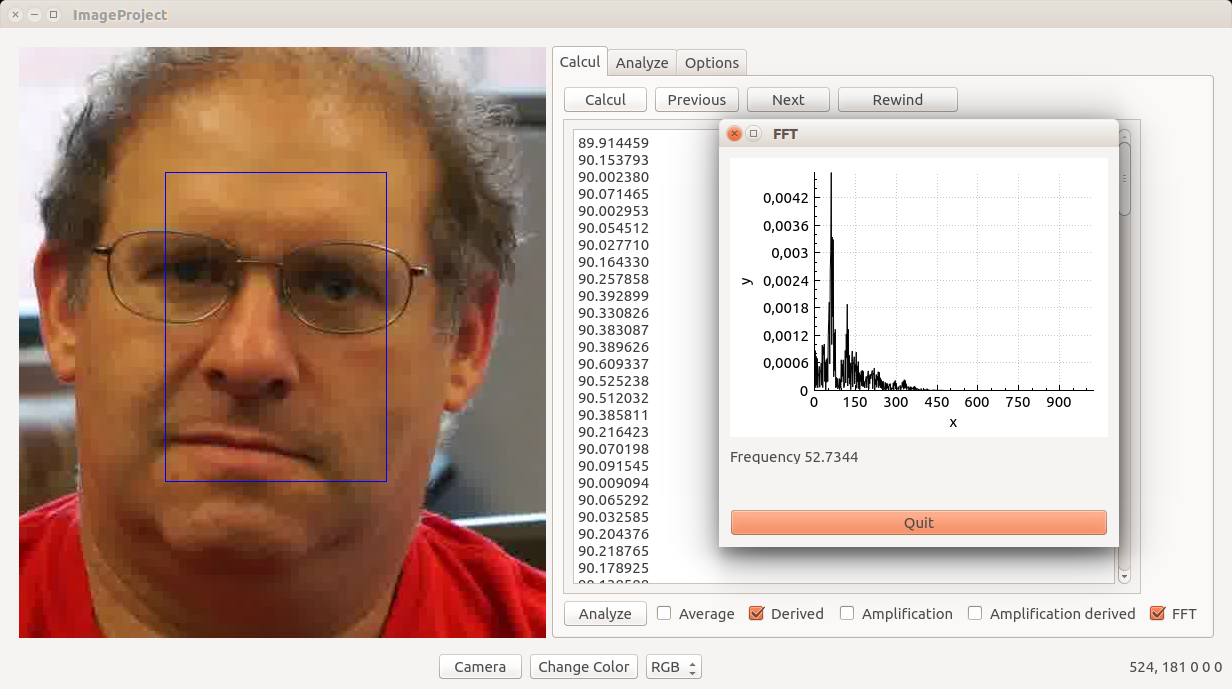
\includegraphics[width=0.9\textwidth]{data/cas-ideal.png}
	\caption{Vidéo source du MIT analysé avec notre logiciel.}
\end{figure}

On pouvait se poser la question, des personnes de couleur, est-ce qu'une couleur de peau différente aurait pu avoir des conséquences? Nous avons
donc tester avec une autre vidéo fournie par le MIT avec une personne de peau noir, on peut voir sur la capture suivante que cela n'a en rien influencer
sur notre algorithme. On retrouve donc une fréquence comprise entre 47 et 59 BPM\@.

\begin{figure}[h!]
	\centering
	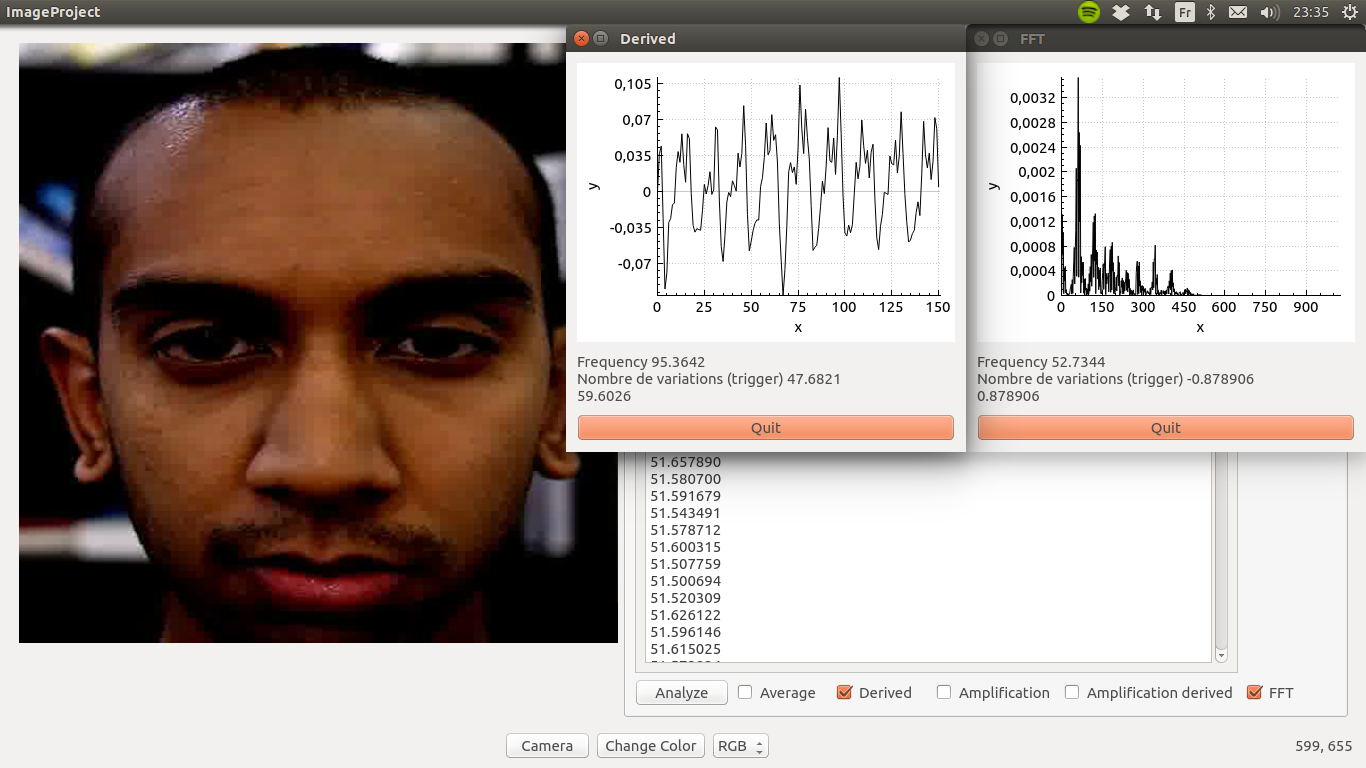
\includegraphics[width=0.9\textwidth]{data/logi.png}
	\caption{Autres test avec une personne de couleur de peau différente.}
\end{figure}


\section{Webcam}

Avec une webcam, nos résultats sont moins précis, mais sont assez correct pour être utiliser. 

\begin{figure}[h!]
	\centering
	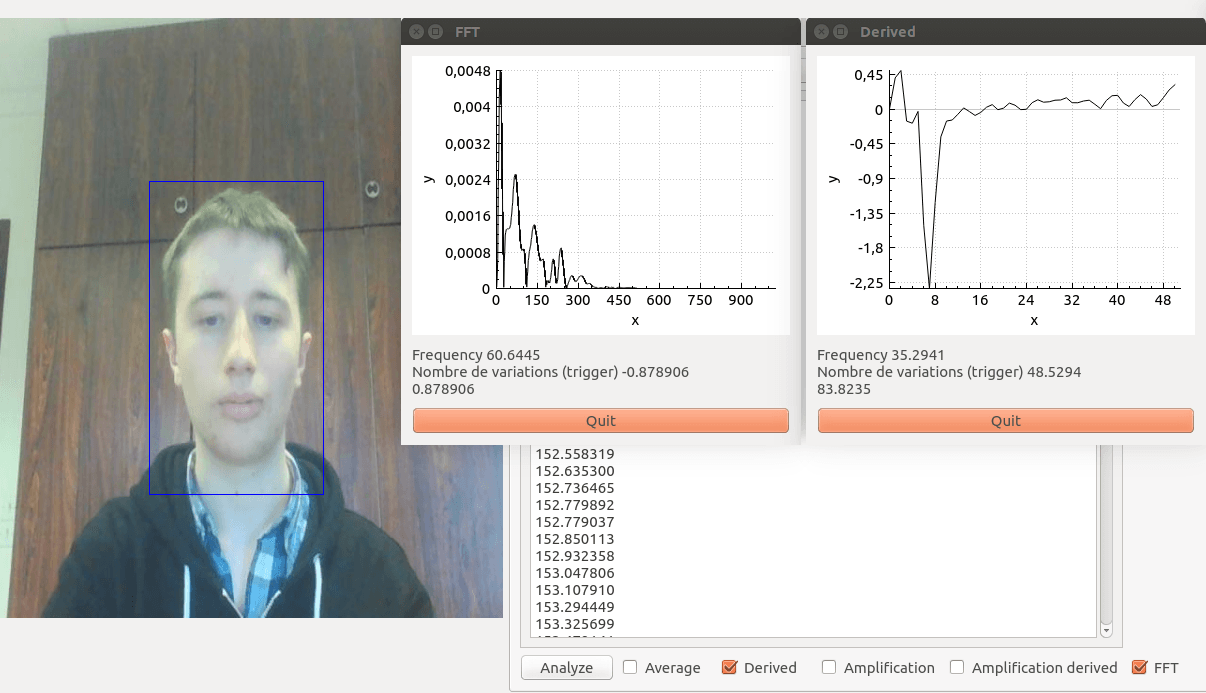
\includegraphics[width=1\textwidth]{data/webcam.png}
	\caption{Vidéo pris par la webcam et analysé avec notre logiciel.}
\end{figure}

\section{Mobile}

\subsection{Android}

Notre plus gros problème a était lors de nos tests sur Android, la stabilité de la vidéo et le nombre de frames capturés.
Actuellement notre application est capable de capturer des frames et appliquer notre algorithme mais nos résultats restent erronées.

\subsection{OpenCV}
L'utilisation d'une FFT et d'un Trigger permet de mieux différencier l'homme de la photo. Même si les résultats sont meilleurs il reste de nombreuses erreurs et le temps de calcul est beaucoup plus long.

\subsection{Ressources utilisées}
La mémoire accordé à notre application par le système d'exploitation de l'ordinateur est fixe et ne peut être augmenté.\\
Donc nous devons faire nos enregistements avec une mémoire limitée, c'est à dire que le nombre d'image capturée était limité. Une plus grand resolution de la caméra implique donc moins d'images à enregistrer. \\
De plus le nombre d'opération a effectué étant important, nous avions un temps de calcul assez important sous OpenCV\@. Pour 10 secondes d'enregistement avec une résolution de 480*320 à raison de 6 images par seconde, soit 60 images nous obtenions un temps de calcul de 20 secondes. Ce qui es beaucoup trop important pour une application qui se veut rapide.\\
Sous android natif le problème fut que le nombre d'images capturé n'était pas suffisant pour permettre une analyse correcte, un enregistement d'un nombre trop important d'image (supérieur à 30) engendrait un crash de notre application.



\section{Bilan}

Notre différenciation entre un humain et une photo fonctionne correctement dès lors où la stabilité est assurée. En effet, prenons Android, nous arrivons
à capturer plus de frames qu'en utilisant OpenCV, toutefois le tracking d'OpenCV est plus efficace. De ce fait, malgré une meilleure capture sous Android 
comme la stabilité est plus mauvaise, nos résultats sont moins bons. Mais à contrario, lorsqu'on utilise l'application réalisée avec OpenCV, le nombre d'images
capturé est seulement de 20 pour 4 secondes, avec si peu d'images à traiter notre magnification n'est pas correcte. C'est seulement au bout de 10 secondes
lorsqu'on capture entre 50 à 70 frames qu'on a des résultats cohérents. 



\chapter{Conclusion}
\section{Apports techniques}

Ce projet nous a permis de mettre en œuvre l'enseignement que nous a donné l'ENSICAEN, l'utilisation de Github, les cours de Java/C++ et de conception d'interface graphique. Il nous a également permis d'
apprendre le développement mobile et l'utilisation de librairie comme OpenCV\@.

\subsection{Android}
	Android est un système d'exploitation sur lequel nous n'avions jamais programmé, l'appréhender par nous même fut difficile.
	Le placement des widgets sur l'écran et même le système d'activité, nous étaient inconnus et nous avions passé de nombreuses heures à le comprendre complètement.
	De plus notre projet utilse la caméra, l'un des périphériques, le plus difficile à mettre en place.

	L'un des plus gros avantages d'android, c'est la documentation qui est bien écrite, ce qui est très appréciable. Grâce à ce projet, nous avons pu avoir un aperçu du système, de ces forces et
	de ces faiblesses.

\subsection{Qt}
	Nous avons déjà eu quelques expériences avec cette bibliothèque, mais nous avons réellement pu appliquer nos connaissances avec ce projet.
	Notre logiciel de test fut d'une grande aide pour l'intégration de nos algorithmes sous Android.\\
	Ce logiciel comprenant de nombreux modules, nous avons dû appliquer des méthodes vue en génie logiciel pour que celui-ci fonctionne correctement.

\subsection{OpenCV}
Nous avons dû utiliser la bibliothèque OpenCV, ce qui était une nouveauté. Celle ci nous a permis d'avoir un meilleur contrôle des images prises par la webcam.

\section{Apports scientifiques}

Nous avons également pu mettre à profit les cours que nous avons eus sur les différents espaces de couleurs, surtout utiles comme nous l'avons vu lors du développement Android.
Le plus gros défi fut la mise en place de techniques du traitement du signal, telle que la FFT ou encore la réalisation d'un filtre basse fréquence.

\section{Bilan}

Ce projet a donc été un vrai aboutissement de notre formation. Il nous a forcé à appréhender de nouvelles technologies et librairies mais également à réutiliser tout ce que nous
 connaissions. Nous avons pu voir les nombreux avantages d'une documentation bien construite et bien imagée, cela permettant de bien sur s'approprier rapidement la technologie étudiée.


\end{document}
